% !TeX document-id = {7077d422-3bd7-43a8-9d95-58f58c3cd9b2}
% !TEX encoding = UTF-8 Unicode
% !TEX TS-program = arara
% arara: lualatex
% arara: clean: {files:[phonphoncomp.bbl,phonphoncomp.blg,phonphoncomp.log,phonphoncomp.aux,phonphoncomp.nav,phonphoncomp.out,phonphoncomp.snm,phonphoncomp.synctex.gz,phonphoncomp.toc]}

\documentclass[12pt,border=0.5cm]{standalone}
\usepackage{fontspec}
\setmainfont[BoldFont=CharisSIL-Bold.ttf,ItalicFont=CharisSIL-Italic.ttf]{CharisSIL-Regular.ttf}
\usepackage{tikz}
\usetikzlibrary{arrows,automata,positioning}

\begin{document}

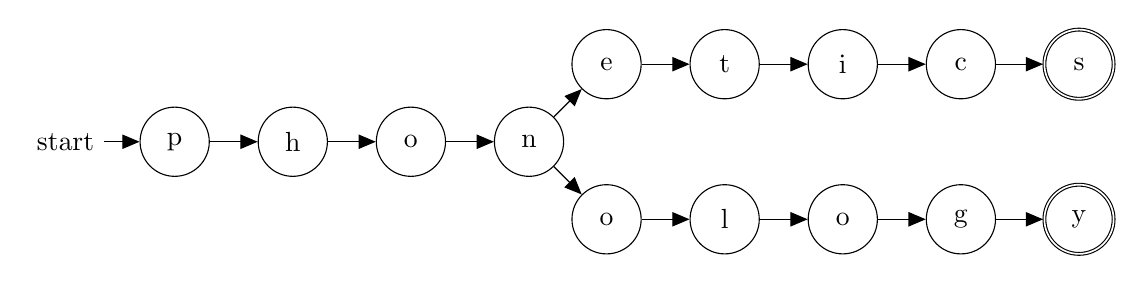
\begin{tikzpicture}[>=triangle 45,node distance = 1.5cm]
\node[state,initial]  (q0)   {p};
\node[state, right of=q0] (q1) {h};
\node[state, right of=q1] (q2) {o};
\node[state, right of=q2] (q3) {n};
\node[state, above right= 0.5cm of q3] (q4) {e};
\node[state, below right= 0.5cm of q3] (q5) {o};
\node[state, right of=q4] (q6) {t};
\node[state, right of=q6] (q7) {i};
\node[state, right of=q7] (q8) {c};
\node[state, right of=q8, accepting] (q9) {s};
\node[state, right of=q5] (q10) {l};
\node[state, right of=q10] (q11) {o};
\node[state, right of=q11] (q12) {g};
\node[state, right of=q12, accepting] (q13) {y};
\path[->]  (q0) edge (q1) 
               (q1) edge (q2)
               (q2) edge (q3)
               (q3) edge (q4)
               (q3) edge (q5)
               (q4) edge (q6)
               (q6) edge (q7)
               (q7) edge (q8)
               (q8) edge (q9)
               (q5) edge (q10)
               (q10) edge (q11)
               (q11) edge (q12)
               (q12) edge (q13);
\end{tikzpicture}

\end{document}

